\input{beamer_annales.sty}


%\usepackage[utf8]{inputenc}
\mode<presentation>
{
	\usetheme{Warsaw}
	\setbeamercovered{transparent}
}


\usepackage{appendixnumberbeamer}
\usepackage{times}

\usepackage{graphicx}
\usepackage{capt-of}
\usepackage{booktabs}
\usepackage{varwidth}

\newcommand\Fontvi{\fontsize{8}{8.2}\selectfont}

\usepackage{appendixnumberbeamer}

\usepackage[]{algorithm2e}

\usepackage{booktabs}

\usepackage[scale=2]{ccicons}

\usepackage{pgfplots}
\usepgfplotslibrary{dateplot}
\pgfplotsset{compat=1.16}

\usepackage{mathtools}
\DeclarePairedDelimiter{\ceil}{\lceil}{\rceil}

\usepackage{xspace}
\newcommand{\themename}{\textbf{\textsc{metropolis}}\xspace}

\title[Asymptotics on the Lempel-Ziv 78 compression of Markov sources]
{Asymptotics on the Lempel-Ziv 78 compression of Markov sources}

\subtitle
{Découverte de la théorie analytique de l'information,
échantillonnage de processus de Markov et preuves
d'analyse combinatoire}

\author[Duboc]
{Guillaume~Duboc}

\institute[
	Universities of Somewhere and Elsewhere]
{
	Département d'informatique\\
	Ecole Normale Supérieure de Lyon}

\date[M1 2018]
{Stage de recherche de M1, 2018}

\subject{Informatique Fondamentale}

\pgfdeclareimage[height=0.5cm]{logoENS}{../latex-figures/presentation-figures/logoENS.png}
\logo{\pgfuseimage{logoENS}}

% \date{\today}
% \titlegraphic{\hfill\includegraphics[height=0.5cm]{../latex-figures/presentation-figures/logoENS.png}}
\AtBeginSubsection[]
{
	\begin{frame}<beamer>[noframenumbering]{Table des matières}
	\tableofcontents[currentsection,currentsubsection]
\end{frame}
}


\expandafter\def\expandafter\insertshorttitle\expandafter{%
% \insertshorttitle\hfill%
\insertframenumber\,/\,\inserttotalframenumber}

\usepackage{caption}
\setbeamertemplate{caption}[numbered]


\makeatletter
\let\@@magyar@captionfix\relax
\makeatother

\begin{document}

\maketitle

\begin{frame}{Table des matières}
  \tableofcontents
\end{frame}


\section{Problème initial : compression de données}
\subsection{Sources d'information}

\begin{frame}{Source probabilistes}
	\begin{block}{Définition: source d'information}
		Soit $\mathcal{A}$ un alphabet. Une \emph{\bfseries source d'information} 
		est une suite infinie de variables aléatoires $X_k$, pour $k\in\Nstar$ :
		\centers{$ X = X_1 X_2 X_3 \dots $}
		où chaque $X_k$ sélectionne un symbole de $\mathcal{A}$.
	\end{block}

	\begin{block}{Définition : source de Markov}
		Une \emph{\bfseries source de Markov} est une source d'information
		pour laquelle la dépendance entre les variables $X_k$ est \emph{markovienne}.
		On parle de source d'\emph{\bfseries ordre $r$} si la probabilité d'occurrence d'un
		symbole dépend uniquement des \emph{$r$ symboles précédents}.
	\end{block}
\end{frame}


\subsection{Algorithmes de compression}

\begin{frame}{Compression d'information}
	\begin{block}{Définition : schéma de compression}
		Un \emph{\bfseries schéma de compression} est un couple de fonctions 
		sur les mots $(\mathcal{C}, \mathcal{D})$ \textit{i.e.} un
		algorithme de compression et de décompression.
	\end{block}

	\begin{block}{Définition : compression sans pertes}
		\label{def:lossless}
		La compression \emph{\bfseries sans pertes} restaure l'information compressée
		dans son état d'origine. Pour tout mot $w$
		\centers{$\mathcal{D}(\mathcal{C}(w)) = w $}
	\end{block}
\end{frame}


% \begin{frame}
% 	\begin{block}{Elements description}
% 		The data representation is $(\text{dictionary\_reference}, \text{symbol})$.
% 	\end{block}

% 	\begin{block}{Remarks}
% 		The LZ78 algorithm builds a prefix tree from which the original word
% 		can be reconstructed.
% 	\end{block}
% \end{frame}

\begin{frame}{Algorithme 1998}

	\begin{block}{Exemple de compression LZ'78}
		\centers{$w = 11001010001000100$}
		\centers{(1)(10)(0)(101)(00)(01)(000)(100)}
		\centers{$([0, '1'], [1, '0'], [0, '0'], [2, '1'],
							[3, '0'], [3, '1'], [5, '0'], [2, '0'])$}
	\end{block}

		\centers{
		$\mathcal{T}(w)$
			 \begin{minipage}{0.55\textwidth}
			 	\centers{
			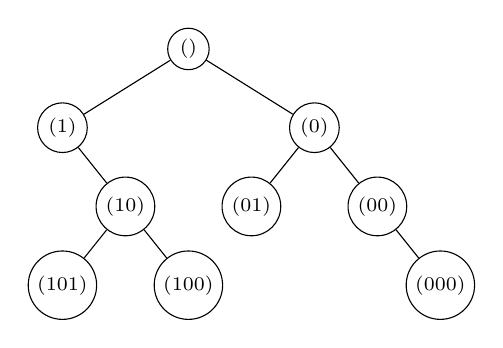
\begin{tikzpicture}[
				level 1/.style={level distance=10mm,sibling distance=32mm},
				level 2/.style={level distance=10mm,sibling distance=16mm},
				level 3/.style={level distance=10mm,sibling distance=16mm},
				font=\scriptsize,inner sep=2pt,every node/.style={draw,circle,minimum size=3ex}]
			]
			\node {()}
				child {node {(1)}
					child[missing]
					child {node {(10)}
						child {node {(101)}}
						child {node {(100)}}
					}
				}
				child {node {(0)}
					child {node {(01)}}
					child {node {(00)}
						child[missing]
						child {node {(000)}}
					}
				}
					;
			\end{tikzpicture}
			}
			\end{minipage}
			$M(w) = 8$
		}
	\end{frame}


\begin{frame}
	\begin{block}{Notation : paramètre du nombre de phrases}
		Le \emph{nombre de phrases} générées par la compression 
		d'un mot $w$ de taille $n$ est noté $M_n(w)$. 
	\end{block}

	\begin{block}{Longueur du code}
		Le code du mot $w$ est de taille :
		\centers{$ |C(w)| = 
					\Sum{k=0}{M(w)} 
					\left( 
						\ceil{\log_2(k)} 
						+ \ceil{\log_2(\mathcal{A})} 
					\right) $}
	\end{block}
\end{frame}

\subsection{Étude asymptotique}

\begin{frame}

	\begin{block}{Définition : taux de compression}
		Le \emph{\bfseries taux de compression} $\tau_n$ est la moyenne divisée par $n$
		des tailles des codes des textes de taille $n$.
		\centers{$ \tau_n = \f{E[C_n]}{n}$}
	\end{block}

	\begin{block}{Remarque}
		Une compression est efficace dès que l'on a $\tau_n < 1$.
	\end{block}

\end{frame}

\begin{frame}{Entropie}
	\begin{block}{Entropie d'une source d'information}
		On définit $X_n$ la variable aléatoire d'un 
		texte généré par une source d'information.

		L'entropie de $X_n$ est 
		\centers{$ h(X_n) = -\Sum{\text{texte}}{}\Pr(\text{texte})\log\Pr(\text{texte})$}

		L'entropie de la source est 
		\centers{$ h = \underset{n\rightarrow\pinf}{\limt} (h(X_{n+1}) - h(X_n)) $}
	\end{block}
\end{frame}

\begin{frame}{Optimalité et redondance}

	\begin{block}{Compression optimale}
		Un algorithme de compression est dit \emph{optimal} si le taux 
		de compression est exactement égal à l'entropie.
		Il est  
		\emph{asymptotiquement optimal} s'il converge vers l'entropie
		pour des textes de taille croissante.
	\end{block}

	\begin{block}{Compression universelle}
		Un algorithme est dit \emph{universel} si sa mise en oeuvre ne nécessite 
		pas de connaissances \textit{a priori} sur la distribution de la source 
		à compresser.
	\end{block}

\end{frame}

\begin{frame}

	\begin{block}{Dans la pratique}
		Le compromis entre optimalité et vitesse de compression/décompression 
		est un problème d'ingénierie tout à fait actuel.
		\begin{itemize}
			\item Google (Brotli, 2015)
			\item Facebook (Zstandard, 2016)
			\item Dropbox (DivANS, 2018)
		\end{itemize}
	\end{block}

\end{frame}

	\begin{frame}{Optimisations}

		\begin{block}{Vitesse de convergence}
			Sur des textes simples pour LZ'78
			\centers{$\tau_n - h = \grando \left( \f{1}{\log \, n} \right)$}
		\end{block} 

		\begin{block}{Algorithmes de partitionnement optimal}
			Famille d'algorithmes consistant 
			à modifier le processus de sélection des phrases de LZ'78 
			pour améliorer la \emph{vitesse de convergence du
			taux de compression vers l'entropie}.

			Exemple : \emph{Flexible parsing}.
		\end{block}
	\end{frame}

% \begin{frame}{ Optimal encoding }
% 	\begin{block}{ Entropy of a Markov source }
% 		Let $\pi$ be a stationary distribution. 
% 		The entropy of a Markov chain is 
% 		\centers{$ h = - \Sum{i=1}{V} \pi \Sum{j=1}{V} p_{i j} \log(p_{i j}) $}
% 	\end{block}

% 	\begin{block}{ Optimality of LZ78 }
% 		Considering words of length $n$.

% 		\centers{$ \f{|C(w)|}{|w|} -h$ goes to zero for $n \rightarrow \pinf$}
% 	\end{block}
% \end{frame}

% \subsection{Algorithmic improvements }
% 	\begin{frame}{ Optimal parsing}
% 	\end{frame}
% 	\begin{frame}{ Flexible parsing }
% 	\end{frame}

\section{Architecture de la solution}
\subsection{Simulation des modèles probabilistes}


{\setbeamercolor{background canvas}{bg=white}
\begin{frame}{Modèle des séquences de Markov indépendantes}

	\begin{block}{Exemple de séquences}
		$\begin{array}{cl}
		X(1) &= 00000\dots \\
		X(2) &= 1010101\dots \\
		X(3) &= 1001101\dots \\
		X(4) &= 001100111\dots \\
	    \end{array}$
	\end{block}

	\begin{block}{Phrases obtenues}
		\centers{$(0)(1)(10)(00)$}
	\end{block}

\end{frame}}

\subsection{Implémentation}

\begin{frame}
	\begin{block}{Sources probabilistes}
		\begin{itemize}
			\item[] {\color{gray} markov.py } 
			\item[] \quad Implémentation des sources de Markov. 
			\item[] {\color{gray} parallel\_tails.py} 
			\item[] \quad Génération rapide et parallélisée de séquences.
		\end{itemize}
	\end{block}

	\begin{block}{Algorithme}
		\begin{itemize}
			\item[] {\color{gray} lempelziv.py} 
			\item[] \quad Compression Lempel-Ziv'78.
		\end{itemize}
	\end{block}
\end{frame}

\begin{frame}
	\begin{block}{Résultats et visuels}
		\begin{itemize}
			\item[] {\color{gray} neininger.py  szpan.py  eigenvalues.py  normal.py} 
			\item[] \quad Calcul d'expressions théoriques.
			\item[] {\color{gray} main.py  tails.py} 
			\item[] \quad Tracé de graphes.
			\item[] {\color{gray} experiments.py  experiment\_tails.py} 
			\item[] \quad Maintenance des jeux de données.
		\end{itemize}
	\end{block}
\end{frame}


\subsection{Visualisations}

\begin{frame}
	\begin{block}{Théorème
		centrale limite}
        Le paramètre $M_n$ obéit a une 
		\emph{\bfseries loi centrale limite} au sens où 
		sa distribution est \emph{\bfseries normale asymptotique}.
        C'est à dire, pour $x = \grando(1)$
        
          \centers{$ \underset{n\rightarrow\pinf}{\limt}
          \proba{} \left\{ \f{M_n-E[M_n]}{\sqrt{\Var[M_n]}} \leq x \right\}
              = \f{1}{\sqrt{2\pi}} \Int{\minf}{x} 
                                      \ex{-\tf{t^2}{2}}\dt$}
	\end{block}
	
	\begin{block}{Remarque}
		\label{rmk:clt}
		Ce théorème
		est un probleme ouvert depuis 20 ans.
	\end{block}
\end{frame}

\begin{frame}
	\begin{figure}
		\centering
		\includegraphics[height=0.69\textheight, width = 0.75\textwidth,
								trim = 26.7cm 0 0 2cm,
								clip=true]{./figs/empirical_normalization_10e6_500.png}
		\centering
		\captionsetup{justification=centering,margin=2cm}
		\caption{Standardized $M_n$ distribution \textit{v.s.} normal distribution\\
			$n_{\text{exp}} = 500, n_{\text{word}} = 10^6$}
		\label{fig:normalized}
	\end{figure}
\end{frame}

\begin{frame}
	\begin{figure}[H]
		\centering
		\includegraphics[height=0.69\textheight, width = 0.75\textwidth,
							trim = 27cm 0 0 2cm,
								clip=true]{./figs/cdf_1e6_500.png}
		\captionsetup{justification=centering,margin=2cm}
		\caption{CDF of standardized $M_n$ vs. normal law\\
				$n_{\text{exp}} = 500, n_{\text{word}} = 10^6$}
		\label{fig:cdf}
	\end{figure} 
\end{frame}

\begin{frame}
	\begin{block}{Théorème
		centrale limite}
        Le paramètre $M_n$ obéit une 
		\emph{\bfseries loi centrale limite} au sens où 
		sa distribution est \emph{\bfseries normale asymptotique}.
        C'est à dire, pour $x = \grando(1)$,
        
          \centers{$ \underset{n\rightarrow\pinf}{\limt}
          \proba{} \left\{ \f{M_n-E[M_n]}{\sqrt{\Var[M_n]}} \leq x \right\}
              = \f{1}{\sqrt{2\pi}} \Int{\minf}{x} 
                                      \ex{-\tf{t^2}{2}}\dt$}
	\end{block}
	
	\begin{block}{Remarque}
		\label{rmk:clt}
		Ce théorème
		est un problème ouvert depuis 20 ans.
	\end{block}
\end{frame}

\begin{frame}{Hypothèses d'expressions pour la variance}

		\begin{block}{Définition : valeur propre}
			On définit $\lambda(s)$ la valeur propre de plus 
			grand module de la matrice
			\centers{
			$P(s) =
			\left\{
			\begin{array}{ll}
				{p_{1 1}}^{-s} & {p_{1 2}}^{-s} \\
				{p_{2 1}}^{-s} & {p_{2 2}}^{-s} 
			\end{array}
			\right\}
			$}
			
		\end{block}

		\begin{block}{Variance}
			La variance dont on vérifie la plausibilité est  
			\centers{$ \Var[M_n] =  \left( \ddot{\lambda}(-1) - { \dot{\lambda}(-1) }^2 \right) \f{n}{\ln^2 n} $}
		\end{block}
\end{frame}

\begin{frame}
	\begin{figure}
		\centering
		\includegraphics[height=0.69\textheight, width = 0.85\textwidth,
							trim = 15 0 20cm 1.2cm,
								clip=true]{./figs/std_analysis_2e4_500.png}	
		\captionsetup{justification=centering,margin=2cm}
		\caption{Variance théorique ${V_n}$ comparée à la variance empirique\\
				$n_{\text{exp}} = 500$}
		\label{std_nein}
	\end{figure} 
\end{frame}

\begin{frame}
	\begin{figure}
		\centering
		\includegraphics[height=0.69\textheight, width = 0.85\textwidth,
							trim = 0 0 16.5cm 1.0cm,
								clip=true]{./figs/eig_fig1.png}	
		\captionsetup{justification=centering,margin=2cm}
		\caption{Comportements asymptotiques des déviations standards\\
					$n_{\text{exp}} = 400$}
	\end{figure}
\end{frame}

\begin{frame}
	\begin{figure}[H]
		\centering
		\includegraphics[height=0.69\textheight, width = 0.85\textwidth,
								trim = 0 0 0 0,
									clip=true]{./figs/eig_fig5.png}	
		\captionsetup{justification=centering,margin=2cm}
		\caption{Comportements asymptotiques des déviations standards\\
				$10^6 \leq n_{\text{word}} \leq 5\cdot 10^6, n_{\text{exp}}=200$}
	\end{figure}
\end{frame}


\begin{frame}
\begin{figure}[H]
		\centering
		\includegraphics[height=0.69\textheight, width = 0.85\textwidth,
								trim = 0 0 0 0,
									clip=true]{./figs/eig_fig4.png}	
		\captionsetup{justification=centering,margin=2cm}
		\caption{Comportements asymptotiques des déviations standards\\
		$10^7 \leq n_{\text{word}} \leq 2\cdot10^7, n_{\text{exp}}=100$}
	\end{figure}
\end{frame}

	% \begin{frame}
	% 	\includegraphics[height=0.69\textheight, width = 0.75\textwidth]{./figs/eig_fig1.png}
	% \end{frame}

\section{Théorie analytique de l'information}

\subsection{Motivation}

	\begin{frame}
		\begin{block}{Calcul de l'entropie}
			\begin{itemize}
				\item La qualité des algorithmes de compression s'apprécie 
			quand les tailles des textes à compresser sont grandes.
				\item L'entropie borne le taux de compression possible.
				\item La compression permet d'estimer l'entropie d'une 
				source \textit{a posteriori}.
			\end{itemize}
		\end{block}

		\begin{block}{Méthode analytique}
			\begin{itemize}
				\item Techniques puissantes issues de l'analyse complexe.
				\item Développements asymptotiques précis.
			\end{itemize}
		\end{block}
	\end{frame}



\subsection{Lèmmes de poissonisation}

\begin{frame}
	\begin{block}{Séries génératrices de Poisson}
		
		\centers{$ A(z) = \Sum{n}{} a_n \f{z^n}{n!} \ex{-z}$}
		
		\begin{itemize}
			\item adaptés à la manipulation des variables aléatoires
		liées à la combinatoire
			\item dépendences croisées (sources de Markov)
		\end{itemize}
	\end{block}

	\begin{block}{P. Jacquet et W. Szpankowski}
		Théorèmes permettant le passage
		\centers{
		étude asymptotique de ces séries complexes
		$\rightarrow$
		développements asymptotiques des suites de coefficients
		}
	\end{block}

\end{frame}

\subsection{Étude d'un paramètre}

\begin{frame}
	\begin{block}{Preuve du théorème central limite}
		L'analyse de la covariance
		\centers{$\Cov(T_n^{\,0}, L_n^{\,0})$}
		est un des jalons de la preuve du théorème central
		limite.
	\end{block}

	
\end{frame}

\begin{frame}{Visualisation} \begin{figure}
	\centering
	\includegraphics[height=0.69\textheight, width=\textwidth,
				  trim = 0 0 0 2.8cm,
						  clip=true]
	  {./figs/var2.png}
	\caption{Comportement asymptotique des variances ${T_n}^{0}$ (gauche) et ${L_n}^{0}$ (droite) \\
					$n_{\text{exp}} = 1546$}
	 \label{fig:var}  
  \end{figure}
\end{frame}


\begin{frame}{Visualisation}
	\begin{figure}
	\centering
	\includegraphics[height=0.69\textheight, width=\textwidth,
			  trim = 0 0 0 2.8cm,
					  clip=true]
	  {./figs/cov2.png}
	\caption{Comportement asymptotique de la covariance\\
			$n_{\text{exp}} = 1546$}
	  \label{fig:cov}
	
  \end{figure}
  
 \end{frame}



	\begin{frame}
		\begin{block}{Relation de récurrence trouvée}
			  \centers{$
			  	\Cov(T_{n+1}^{\,c}, L_{n+1}^c) = 
          			\Cov ( {{\tilde T}_{N_a}}^a,
                         {{\tilde L}_{N_a}}^a )
          			+ \Cov ( {{\tilde T}_{N_b}}^b, 
                          {{\tilde L}_{N_b}}^b ) $}
			\end{block}

			\begin{block}{Série de Poisson et équation différentielle}
				On définit \centers{$C_c(z) 
				= \Sum{n\geq0}{} \Cov(T_n^{\,c}, L_n^{\,c}) 
								\f{z^n}{n!} \ex{-z}$}
				
				d'où découle
			\centers{$
				\partial_z C_c(z) + C_c(z) 
					= C_a(zp) + C_b(zq)
			$}
				permettant de dériver le comportement asymptotique 
				de $C_c(z)$ et, après dépoissonisation, de la covariance.
			\end{block}
	\end{frame}

	% \begin{frame}\includegraphics[width=0.75\textwidth]{./figs/cdf_1e6_500.png}\end{frame}
	
	% \begin{frame}\includegraphics[width=0.75\textwidth]{./figs/eig_fig1.png}\end{frame}
	% \begin{frame}\includegraphics[width=0.75\textwidth]{./figs/eig_fig2.png}\end{frame}
	% \begin{frame}\includegraphics[width=0.75\textwidth]{./figs/eig_fig3.png}\end{frame}
	% \begin{frame}\includegraphics[width=0.75\textwidth]{./figs/eig_fig4.png}\end{frame}
	% \begin{frame}\includegraphics[width=0.75\textwidth]{./figs/eig_fig5.png}\end{frame}
	% \begin{frame}\includegraphics[width=0.75\textwidth]{./figs/empirical_normalization_10e6_500.png}\end{frame}
	% \begin{frame}\includegraphics[width=0.75\textwidth]{./figs/mean_analysis_2e4_500.png}\end{frame}
	% \begin{frame}\includegraphics[width=0.75\textwidth]{./figs/M_n_raw_10e6_500.png}\end{frame}
	% \begin{frame}\includegraphics[width=0.75\textwidth]{./figs/mu_and_neininger_10e6_500.png}\end{frame}
	% \begin{frame}\includegraphics[width=0.75\textwidth]{./figs/simple2.png}\end{frame}
	% \begin{frame}\includegraphics[width=0.75\textwidth]{./figs/std_analysis_2e4_500.png}\end{frame}
	% \begin{frame}\includegraphics[width=0.75\textwidth]{./figs/std_analysis2.png}\end{frame}
	% \begin{frame}\includegraphics[width=0.75\textwidth]{./figs/std_analysis_approx_2e4_500.png}\end{frame}
	% \begin{frame}\includegraphics[width=0.75\textwidth]{./figs/var1.png}\end{frame}
	% \begin{frame}\includegraphics[width=0.75\textwidth]{./figs/var2.png}\end{frame}

\begin{frame}{Sommaire}

	\begin{itemize}
		\item La compression de données : outil d'importance cruciale à analyser dans le contexte de la théorie de l'information.
		\item Une approche pratique et théorique permet une bonne compréhension des performances de ces algorithmes.
	\end{itemize}
	\end{frame}

\appendix

\begin{frame}[allowframebreaks]
\nocite{*}
\bibliographystyle{unsrt}
\bibliography{bibzotm}
\end{frame}


\section*{ Application to covariance analysis }

	\subsection*{ Tail symbols }

		\begin{frame}{Tail symbols}

			\begin{block}{ Illustration }
				\begin{egalites}
	& X(1) 
		& {\color{red}{0}} {\color{green}{0}} 00000\dots \\
	&X(2) 
		& {\color{red}{1}} {\color{green}{0}}10101\dots \\
	& X(3) 
		& {\color{red}{10}} {\color{green}{0}} 1101 \dots \\
	& X(4) 
		& {\color{red}{00}} {\color{green}{1}} 100111\dots
	\end{egalites}
			\end{block}

			\begin{block}{Definition}
				Let $c$ be a character from our alphabet $\{ a, b \}$.
				In the case when all the sequences start with a $c$, we 
				define $T_n^{\,c}$ the \emph{number of times $a$ is a tail symbol in 
				the experiment}.
			\end{block}

		\end{frame}

		\begin{frame}{Definition and relation}

			

			\begin{block}{Recurrence}
				For $n \geq 0$, we have :
					\[ \boxed{ T_{n+1}^{\,c} = \delta_a + 
											{{\tilde T}_{N_a}}^a
											+ {{\tilde T}_{N_b}}^b } \]
			\end{block}
		
			\begin{block}{ Notations }
				\begin{itemize}
				\item $\delta_a = 
							\begin{cases} 
								1 & \text{if $a$ is the tail symbol of the
										first sequence}\\
								0 & \text{else} 
							\end{cases}$

				\item $N_a$ is the 
				random variable giving \emph{the size of the left subtree 
				which contains phrases whose second letter is $a$}

				\item ${{\tilde T}_{N_a}}^a$ is the number of 
				times $a$ is a tail symbol for the sequences that were 
				used to  build the subtree with phrases having $a$ as second
				symbol.

				\item $T_0^c$ for all $c$ by convention.
			\end{itemize}
			\end{block}

		\end{frame}

		\begin{frame}{Total path length}

			\begin{block}{Definition}
				Defining $L_n^{\,c}$ as the \emph{total 
				path length of the nodes of the DST that was built with
				MI model with $n$ sequences starting with letter $c$}.
				It is the sum of the lengths of all the prefix phrases.
			\end{block}

			\begin{block}{Recurrence relation}
				For all $n\geq 0$ :

				\[
				\boxed{ 
					L_{n+1}^c = n + 
										{{\tilde L}_{N_a}}^a + 
										{{\tilde L}_{N_b}}^b
				}
				\]
			\end{block}
		\end{frame}


		\begin{frame}{Algorithme 1998: pseudo-code}

				\label{app:lempelziv}

				\SetKw{KwProcedure}{procedure}
				\SetKw{KwReturn}{return}
				\begin{algorithm}[H]
				\KwProcedure \textsc{Encoding}(w)\;
				$\mathcal{T} \leftarrow$ Tree(0)\;
				$k \leftarrow 1$\;
				\While{$w\neq\text{nil}$}{
				$x\leftarrow \textmd{Read}(w)$\;
				$\mathcal{T}' \leftarrow \mathcal{T}$\;
				\While{$\mathcal{T}'.x \neq \text{nil} \& w \neq \text{nil}$}{
					$\mathcal{T}' \leftarrow \mathcal{T}'.x$\;
					$x\leftarrow\textmd{Read}(w)$\;
				}{
					\If{$\mathcal{T}'.x = \text{nil}$}
					{$\mathcal{T}'.x \leftarrow Tree(k)$}
					\Else{$\mathcal{T}'.\$ \leftarrow Tree(k)$
				}
				$k\leftarrow k+1$
				}}
				\KwReturn $\mathcal{T}$
				\caption{Building the LZ'78 parsing tree}
				\end{algorithm}

		\end{frame}

\end{document}
